%=====================================================================
\section{How we validated the simulator}\label{sec:validation}
%=====================================================================
Every later result depends on the simulator, so before using it we checked it in three independent ways:
\begin{enumerate}
  \item \textbf{Physics tests}: compare the simulator with results derived by hand (exact formulas, conservation laws). These catch coding errors.
  \item \textbf{Published numbers}: compare with the numbers printed in three papers. These catch modelling errors (a wrong sign, a missing term, a wrong parameter).
  \item \textbf{Flight data}: compare with measurements from a real flight. This tells us how close the \emph{model itself} is to reality.
\end{enumerate}
All checks are automated tests that run with one command (\texttt{pytest}). At the time of writing, 46 tests pass and 1 is marked as an expected failure (explained in Section~\ref{sec:val-icra}). A script in the \texttt{experiments} folder (\texttt{v0\_validation\_report.py}) also writes all comparisons into one table in \texttt{results/tables}.

\subsection{Layer 1: physics tests against hand-derived results}
Each test sets up a situation whose answer is known exactly, runs the simulator and compares. None of them compares the simulator with another run of itself.
\begin{longtable}{p{0.27\linewidth}p{0.66\linewidth}}
\toprule
Test & Exact reference result \\
\midrule
\endhead
Free fall & With no thrust: $z(t) = z_0 + v_{z0}t - \tfrac12 gt^2$, and horizontal motion at constant speed (agreement to $10^{-9}$). \\
Thrust direction & Tilted drone, no torque: $\ddot{\vect d} = R\vect e_3 f_\Sigma/m - g\vect e_3$, with $R$ built by hand from Euler angles. \\
Hover balance & With $f_i = mg/4$ all derivatives are zero. \\
Torque-free precession & No thrust, no drag: $r$ stays constant and $(p,q)$ rotate at the rate $\lambda = (I^T_{zz}-I^T_{xx})r/I^B_{xx}$ (Euler's equations solved in closed form; agreement to $10^{-8}$). \\
Angular momentum and energy & For a torque-free rigid body the inertial angular momentum $R I\vect\omega$ and the kinetic energy $\tfrac12\vect\omega^\top I\vect\omega$ must stay constant (relative error below $10^{-8}$). \\
Reduced-attitude kinematics & For constant $\vect\omega$: $\vect n(t) = e^{-[\vect\omega]_\times t}\vect n(0)$, computed with the matrix exponential. \\
Yaw spin-up & Rotors 1 and 3 only, equal thrust: $p=q=0$ stay zero and $I^B_{zz}\dot r = 2\kappa_\tau f - \gamma r$, so $r(t) = r_{ss}(1-e^{-\gamma t/I^B_{zz}})$ with $r_{ss} = 2\kappa_\tau f/\gamma$. \\
Integration order & Halving the time step must reduce the error by about $2^4 = 16$ (RK4 is fourth order); the test accepts 12 to 20. \\
Motor lag & Step response $f(t) = u + (f_0 - u)e^{-t/\sigma}$. \\
Saturation rules & Command $\le0$ gives 0; otherwise clipped to $[f_{\min}, f_{\max}]$; a failed rotor gives 0. \\
Paper's equations & An independent transcription of the paper's eqs.~(12) to (14), written with signed propeller speeds instead of thrusts, equals the simulator at 50 random states. \\
IJRR model reduces to ours & Our separate implementation of the IJRR 2016 model (Section~\ref{sec:val-ijrr}), with its extra effects switched off, equals the simulator at 50 random states. \\
Centre-of-mass motion & At the relaxed hover the vertical acceleration is zero and the horizontal acceleration is $g\sqrt{1-n_z^2}/n_z$ (the paper's eqs.~18 to 20). \\
\bottomrule
\end{longtable}

\subsection{Layer 2: published numbers}
\subsubsection{Mueller and D'Andrea, ICRA 2014}\label{sec:val-icra}
This paper uses exactly our model and parameters, so we expect exact agreement up to the digits printed.
\begin{table}[h]
\centering\small
\caption{Our equilibria against Mueller and D'Andrea, ICRA 2014.}\label{tab:val-icra}
\setlength{\tabcolsep}{4pt}
\begin{tabularx}{\linewidth}{>{\raggedright\arraybackslash}p{3.1cm} L r r r}
\toprule
Case & Quantity & Ours & Published & Difference \\
\midrule
Two opposing rotors lost (eqs.~57--59) & $f_1 = f_3$ (N) & 2.453 & 2.45 & +0.10\% \\
 & propeller speed $\Omega_1$ (rad/s) & $-618.6$ & $-619$ & +0.07\% \\
 & $r$ (rad/s) & 30.14 & 30.1 & +0.14\% \\
\midrule
Three rotors lost (eqs.~62--64) & $f_1$ (N) & 5.369 & 5.37 & $-0.02$\% \\
 & propeller speed $\Omega_1$ (rad/s) & $-915.2$ & $-915$ & $-0.02$\% \\
 & $(p, q, r)$ (rad/s) & (14.68, 0, 32.99) & (14.7, 0, 33.0) & $\le0.11$\% \\
 & $\vect n$ & (0.407, 0, 0.914) & (0.41, 0, 0.91) & $\le0.8$\% \\
\midrule
One rotor lost, $\rho = 0.5$ (eqs.~50--53) & $f_1 = f_3$, $f_2$ (N) & 2.040, 1.020 & 2.05, 1.02 & $-0.5$\%, 0\% \\
 & $r$ (rad/s) & 18.81 & 18.89 & $-0.4$\% \\
 & $n_z$ & 0.962 & 0.958 & +0.4\% \\
 & $q$ (rad/s) & 5.37 & 5.69 & $-5.7$\% \\
 & $n_y$ & 0.274 & 0.289 & $-5.1$\% \\
\midrule
Fig.~3 ($\rho$ sweep) & min $\|\vect\omega\|$ (rad/s) at $\rho$ & 18.62 at 0.675 & 19.0 at 0.655 & $-2.0$\%, +3.0\% \\
 & min $f_1$ (N) at $\rho$ & 2.029 at 0.579 & 2.04 at 0.563 & $-0.5$\%, +2.8\% \\
\bottomrule
\end{tabularx}
\end{table}

\paragraph{Reading.} The two-rotor and three-rotor cases agree to every printed digit. The three-rotor case is a strong check because it exercises all gyroscopic and propeller terms with $p\ne0$. In the one-rotor case the thrusts, the yaw rate and $n_z$ agree within 0.5\%, but $q$ and $n_y$ are 6\% lower. We investigated this gap:
\begin{itemize}
  \item Inserting the paper's own published values ($\vect f$, $\vect\omega$) into the paper's own roll equation (its eq.~12) does \emph{not} give zero: it leaves a roll torque of $-0.011$\,N\,m, about 7\% of the torque from rotor 2. So the published one-rotor values are not an exact equilibrium of the paper's own model with its stated parameters.
  \item The published inertias have only two significant figures. Changing each by $\pm0.05\times10^{-3}$ moves our $q$ between 5.07 and 5.69\,rad/s, so the published value lies at the edge of what rounding allows; but the same parameters reproduce the other two cases exactly.
\end{itemize}
We therefore treat this as an inconsistency in that one published case, not as an error in our model. The test for the published $q$ is kept and marked as an expected failure, so the discrepancy stays visible.

\paragraph{Analytic checks.} The paper's closed form for the yaw rate (its eq.~21) equals our solver. Its coupling constant $\bar a$ (eq.~28) equals the $(p,q)$ entry of our numerical Jacobian. Its controllability condition (eqs.~37 to 39) says that with two opposing rotors lost, the roll rate becomes uncontrollable exactly when $\bar a = 0$; our controllability rank drops from 7 to 6 exactly there.

The sweep over the thrust ratio $\rho$ (Figure~\ref{fig:rho}) reproduces the shape of the paper's Fig.~3; the minima agree within 2\% in value and 3\% in location. Both minima are shallow, so their location is sensitive to small differences.

\begin{figure}[h]
\centering
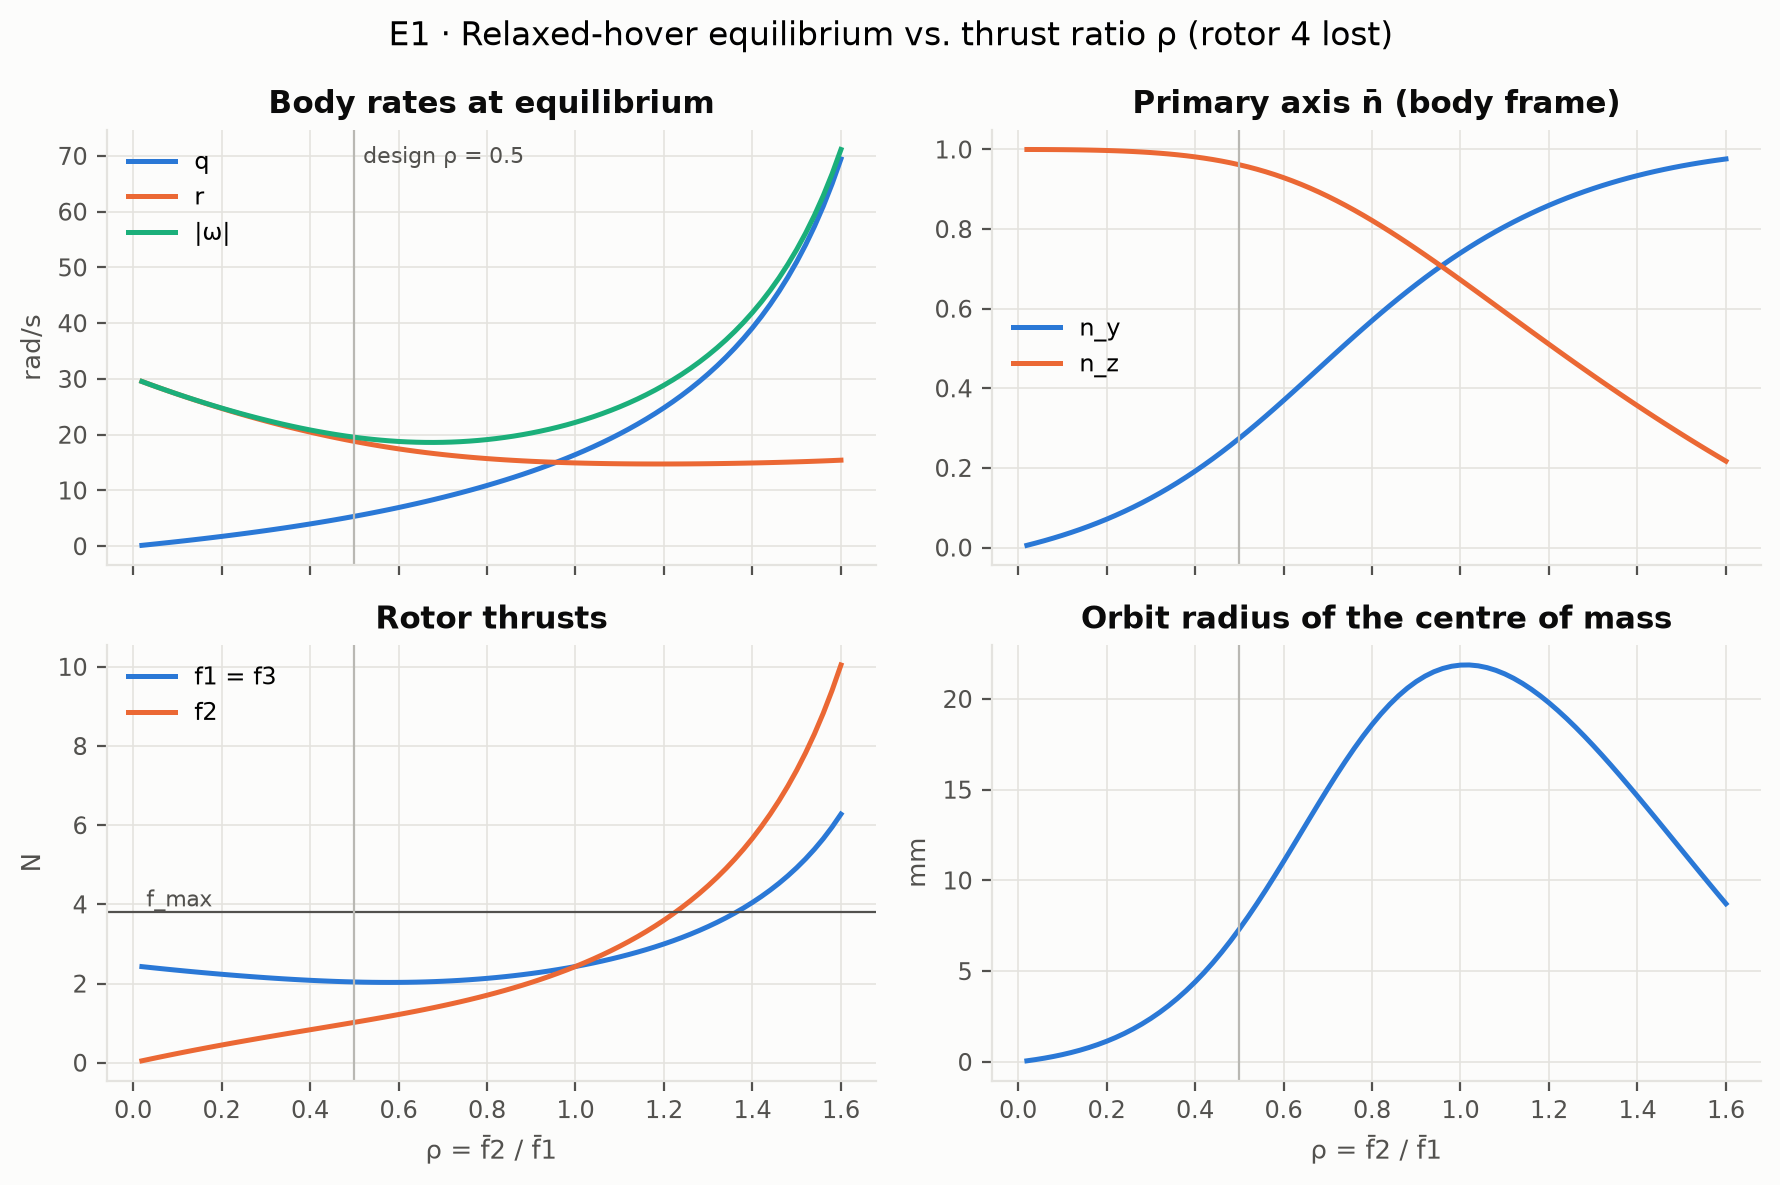
\includegraphics[width=0.85\linewidth]{figures/e1_rho_sweep.png}
\caption{The one-rotor-loss equilibrium as a function of the thrust ratio $\rho = f_2/f_1$ (reproduces the paper's Fig.~3).}\label{fig:rho}
\end{figure}

\subsubsection{Mueller and D'Andrea, IJRR 2016}\label{sec:val-ijrr}
This paper uses the same drone with a more detailed model (air-relative thrust, quadratic drag on all axes, propeller speeds as inputs, the propeller acceleration term kept). To check it we wrote a \emph{separate} implementation, \texttt{validation.py}, deliberately in different variables (propeller speeds instead of thrusts), so that it does not share code with the simulator. For each of the five published cases we give it the published propeller speeds and solve for the body rates at which the rotation stops changing.

\begin{table}[h]
\centering\small
\caption{Hover solutions of IJRR 2016 (Sec.~5.2) against our independent implementation. The last column is $f_\Sigma n_z/(mg)$, which must be 1 at a hover solution.}\label{tab:val-ijrr}
\begin{tabular}{lllll}
\toprule
Case & Published $\Omega$ (rad/s) & Published $\vect\omega$ & Ours & Force ratio \\
\midrule
No failure & (438, 438, 438, 438) & (0, 0, 0) & (0, 0, 0) & 1.003 \\
Rotor 4 lost & (585, 362, 585, 0) & (0.20, 4.30, 19.50) & (0.15, 4.19, 19.47) & 1.002 \\
Rotors 2, 4 lost & (643, 0, 643, 0) & (0, 0, 24.50) & (0, 0, 24.50) & 1.001 \\
Rotors 3, 4 lost & (1067, 218, 0, 0) & (26.00, 0, 23.30) & (24.94, 0.06, 23.57) & 0.995 \\
Rotors 2, 3, 4 lost & (1103, 0, 0, 0) & (28.00, $-1.60$, 24.50) & (26.73, $-1.45$, 24.93) & 0.994 \\
\bottomrule
\end{tabular}
\end{table}

\paragraph{Reading.} With the published parameters, the body-rate vectors agree within 4\% and the force balance within 0.6\%. The two cases with very high rotation rates are the most sensitive to the drag and inertia values, which are printed with one or two significant figures. As a sensitivity check only, $I_{xx} = 2.75\times10^{-3}$ (the upper end of the rounding interval of the printed $2.7\times10^{-3}$) brings all five cases within 0.7\%; because this value was chosen by looking at the same cases, it is not an independent validation.

One number is especially informative. With two opposing rotors lost, the paper's propeller speed is 643\,rad/s at a body spin of 24.5\,rad/s. If thrust depended on the speed relative to the body, $\kappa_f\cdot643^2$ would be 8\% more than $mg/2$; with the speed relative to the air, $\kappa_f(643-24.5)^2 = mg/2$ exactly. So air-relative thrust is real and matters. Our simulator (the ICRA model) does not include it: at the one-rotor equilibrium it would change rotors 1 and 3 by about $-7$\% and rotor 2 by about $+10$\%. This is a known limitation (Section~\ref{sec:discussion}).

\subsubsection{Sun et al., T-RO 2021: a second airframe}
To test the equilibrium solver on a different drone, we used the Parrot Bebop~2 parameters of Sun et al.~\cite{sun2020incremental} (their Table~I in the arXiv version, called Table~III in their text: $m=0.410$\,kg, $l=0.145$\,m, and so on). With two opposing rotors lost, their eq.~(60) gives $\bar r = mg\kappa_\tau/\gamma$ and propeller speed $\sqrt{mg/(2\kappa_f)}$.

\begin{center}\small
\begin{tabular}{lrrr}
\toprule
Quantity & Ours & Eq.~(60) with the parameter table & Printed in the text \\
\midrule
$\bar r$ (rad/s) & 26.81 & 26.81 & 26.4 \\
propeller speed (rad/s) & 1029 & 1029 & 1015 \\
\bottomrule
\end{tabular}
\end{center}
Our solver equals the paper's own formula exactly. The numbers printed in the paper's text are about 1.5\% below its own formula; this difference is internal to the paper.

\subsection{Layer 3: flight data}
\paragraph{Spin-up time.} In the ICRA flight (their Fig.~4), propeller 4 is switched off and the drone flies on propellers 1 and 3 only, without attitude feedback, until the rotation rate reaches 10\,rad/s, which took 0.62\,s. During this phase the roll and pitch torques are zero (rotors 1 and 3 are opposite each other with equal thrust), so only the yaw equation acts:
\begin{equation}
  I^B_{zz}\dot r = 2\kappa_\tau f - \gamma r \quad\Rightarrow\quad r(t) = r_{ss}\big(1 - e^{-\gamma t/I^B_{zz}}\big),\quad r_{ss} = \frac{2\kappa_\tau f}{\gamma},
\end{equation}
so the time to reach 10\,rad/s is $t_{10} = -\frac{I^B_{zz}}{\gamma}\ln\!\big(1 - \tfrac{10}{r_{ss}}\big)$. The answer depends strongly on the thrust $f$ of the two rotors. The paper's text says only that the vehicle ``uses only the two opposing propellers'' during this phase; the thrust is not printed, so we read it from its Fig.~4: rotor 2 is at zero and rotors 1 and 3 at a constant 2.95\,N or so (more than $mg/2 = 2.45$\,N).

\begin{center}\small
\begin{tabular}{lccc}
\toprule
Spin-up thrust & Simulator & Closed form & Flight \\
\midrule
2.95\,N (read from Fig.~4) & 0.65\,s & 0.64\,s & 0.62\,s \\
2.45\,N ($mg/2$) & 0.81\,s & 0.80\,s & not flown \\
\bottomrule
\end{tabular}
\end{center}
At the flight thrust the model is within about 4\% of the flight. Because the thrust is read from a plot, the detection-delay study (Section~\ref{sec:delay}) is reported for both thrusts.

\paragraph{Steady spin rate and height.} The published models over-predict the spin of the real drone. In the ICRA one-rotor flight the measured body rates in hover were $(2.1, 3.7, 13.7)$\,rad/s (their eq.~55), about 14.3\,rad/s against about 19.7\,rad/s predicted by the same model that our simulator implements (ours: 19.6\,rad/s at $\rho = 0.5$), about 27\% less. In the IJRR flight the spin was 15.8\,rad/s against 19.9\,rad/s in simulation (their Sec.~5.4), about 20\% less; those authors suggest extra torques from the motion of the propeller centres as a possible cause. In the ICRA two-rotor flight the drone stayed about 2.4\,m below its set-point, which the authors attribute to the propellers producing less thrust at high body rates. None of these effects is in the nominal model. They are why our truth plants contain a thrust loss at high rotation rate: the learned residual of Section~\ref{sec:koopman} is meant to capture effects of this kind.

\subsection{Summary of the validation}
\begin{plain}
The simulator agrees with the papers wherever the papers are internally consistent, and the only disagreements are explained: one published case that does not satisfy the paper's own equation, two cases whose parameters are printed with very few digits, and two real-world effects (air-relative thrust and thrust loss while spinning) that the paper's own model also leaves out. We can therefore trust the simulator as a faithful implementation of the published model, and we know in which ways the published model differs from the real drone.
\end{plain}
